\chapter{Theorethical Foundations}\label{chapter:theorethical}
\section{Multicore Systems}\label{section:multicore}
Until the beginning of the decade of year 2000 the advances in processor technology were made through improvements in the single CPU performance. These advances allowed the increase in the clock speed of the processors. Given the fact that the heat generated by a transistor is proportional to its operating frequency, the high clock frequencies reached led to a great amount of dissipated heat that could not be easily handled. In order to decrease the consumed power and take advantage of the increasing transistor count in every chip, the industry decided to incorporate multiple CPUs with a moderate performance instead of a single one with a high frequency and therefore power consumption. This new design trend is known as \textbf{multicore}. 

In a single CPU the running code can be executed in a more efficient way by the CPU by using mechanisms such as the reordering of instructions. With the appearance of multicores there is a greater demand on the programmer to write code that can exploit all the available capacity offered by the processor. Part of this increasing programming effort consists of allowing the code to execute in units called \textbf{threads}, where a n core CPU has the capacity to execute n threads simultaneously. This expression of code in threads can be explicitly done with the help of frameworks such as \textit{pthreads} or can be done implicitly by annotating regions of code that can be parallelized using tools such as \textit{OpenMP}.

\subsection{Thread pinning}\label{subsection:pinning}
Given a code that executes in n threads using a processor with m cores, we would like to have the ability to control which executing core will be used to execute a given thread. The mapping of an executing thread to a hardware core is known as \textbf{thread pinning} or \textbf{thread affinity}.

There are many mechanisms available to set the pinning of a program, such as:

\begin{itemize}
	\item In OpenMP the environment variable GOMP\_CPU\_AFFINITY=a,b,c,… sets the affinity of a program as a list where a,b and c represent the identifiers of the cores that will execute the thread with the id in the position in which the identifier was given. In this example thread 0 will be executed in core a, thread 1 in core b and so on.
	\item In numactl the parameter \textit{physcpubind} can specify in a similar manner as is done in OpenMP, as a listing of the desired cores.
	\item In Autopin+ the user specifies many possible pinnings, and the tools will explore these combinations of pinnings for the most optimal in terms of execution speed.
\end{itemize}
Pinning can play a very important role in the performance of a program. In many cases distributing a thread to a free core might yield the best performance, but in other scenarios -especially in NUMA systems- this might not be the case depending of the locations of memory accesses by the thread, these factors will be explored later in more depth. 

\section{The bus interface and multicore systems}\label{section:businterface}
\begin{figure}
	\centering
		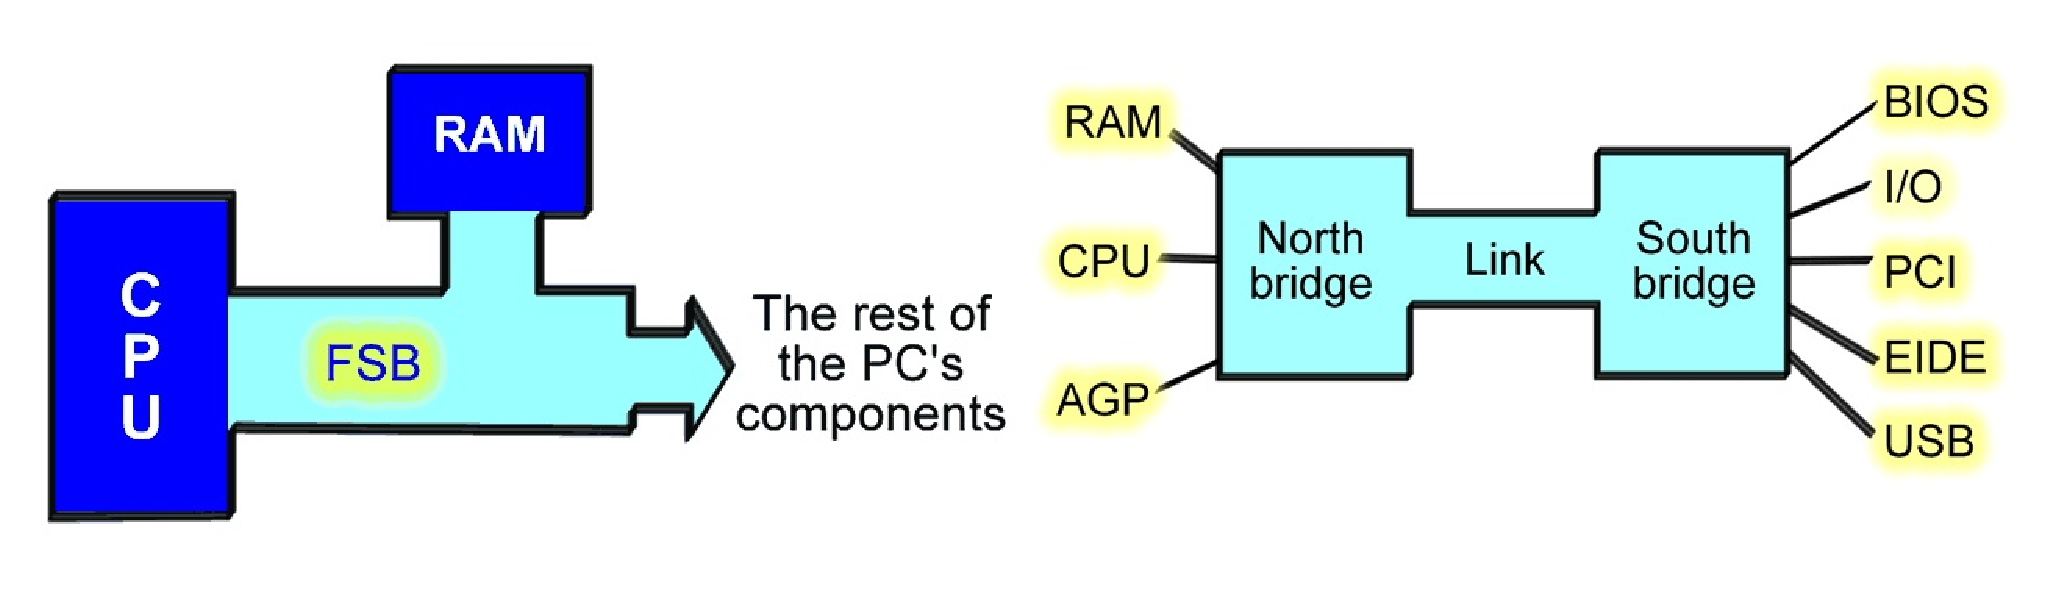
\includegraphics[width=.9\textwidth]{figures/bus-abstraction.eps}
		\caption[bus-abtraction]{Abstraction of the data traffic between the CPU and the external entities. The left hand side abstracts the RAM as being closer to the cpu than the other components, and the right side shows a more accurate description with the Northbridge and Southbridge chips redirecting the traffic. Image Karbosguide \cite{pcarch-carbo}. }
		\label{fig:bus-abs}
\end{figure}

In earlier computer systems, the processor chip had a communication with the memory through a high speed path called the Front Side Bus (FSB), which connects the last level of cache of a processor chip with the memory controller. This Front Side Bus also allows the communication between the processor chip and other peripherals through the Northbridge chip. This layout means that all the traffic between the processor and the exterior world was centralized through the Front Side Bus, but in many cases a great share of the traffic is occupied by the memory-processor data. The visualization of this layout is given in Figure \ref{fig:bus-abs}. 

Given the always present need to optimize the supply of memory data to the CPU, this front side bus scheme has been changed and a quicker way for the CPU to access memory has been devised, these improvements can be seen in the form of higher bandwidth and low latency. Nowadays the path between the processor and the memory controller has been taken in-chip, which means that the processor has a straight path to the memory controller inside the same silicon die. In many modern multicore processors, specifically those from Intel and AMD, every core has its own L1 and L2 caches and all the cores share the L3 or last level cache. With the introduction of the dedicated memory access interface every processor chip has a part not specific to any core which handles the access to memory, in Intel technology this in-chip intermediation area is known as the \textit{uncore}.

\section{Multiprocessor Systems}\label{section:multiproc}

\begin{figure}
	\centering
		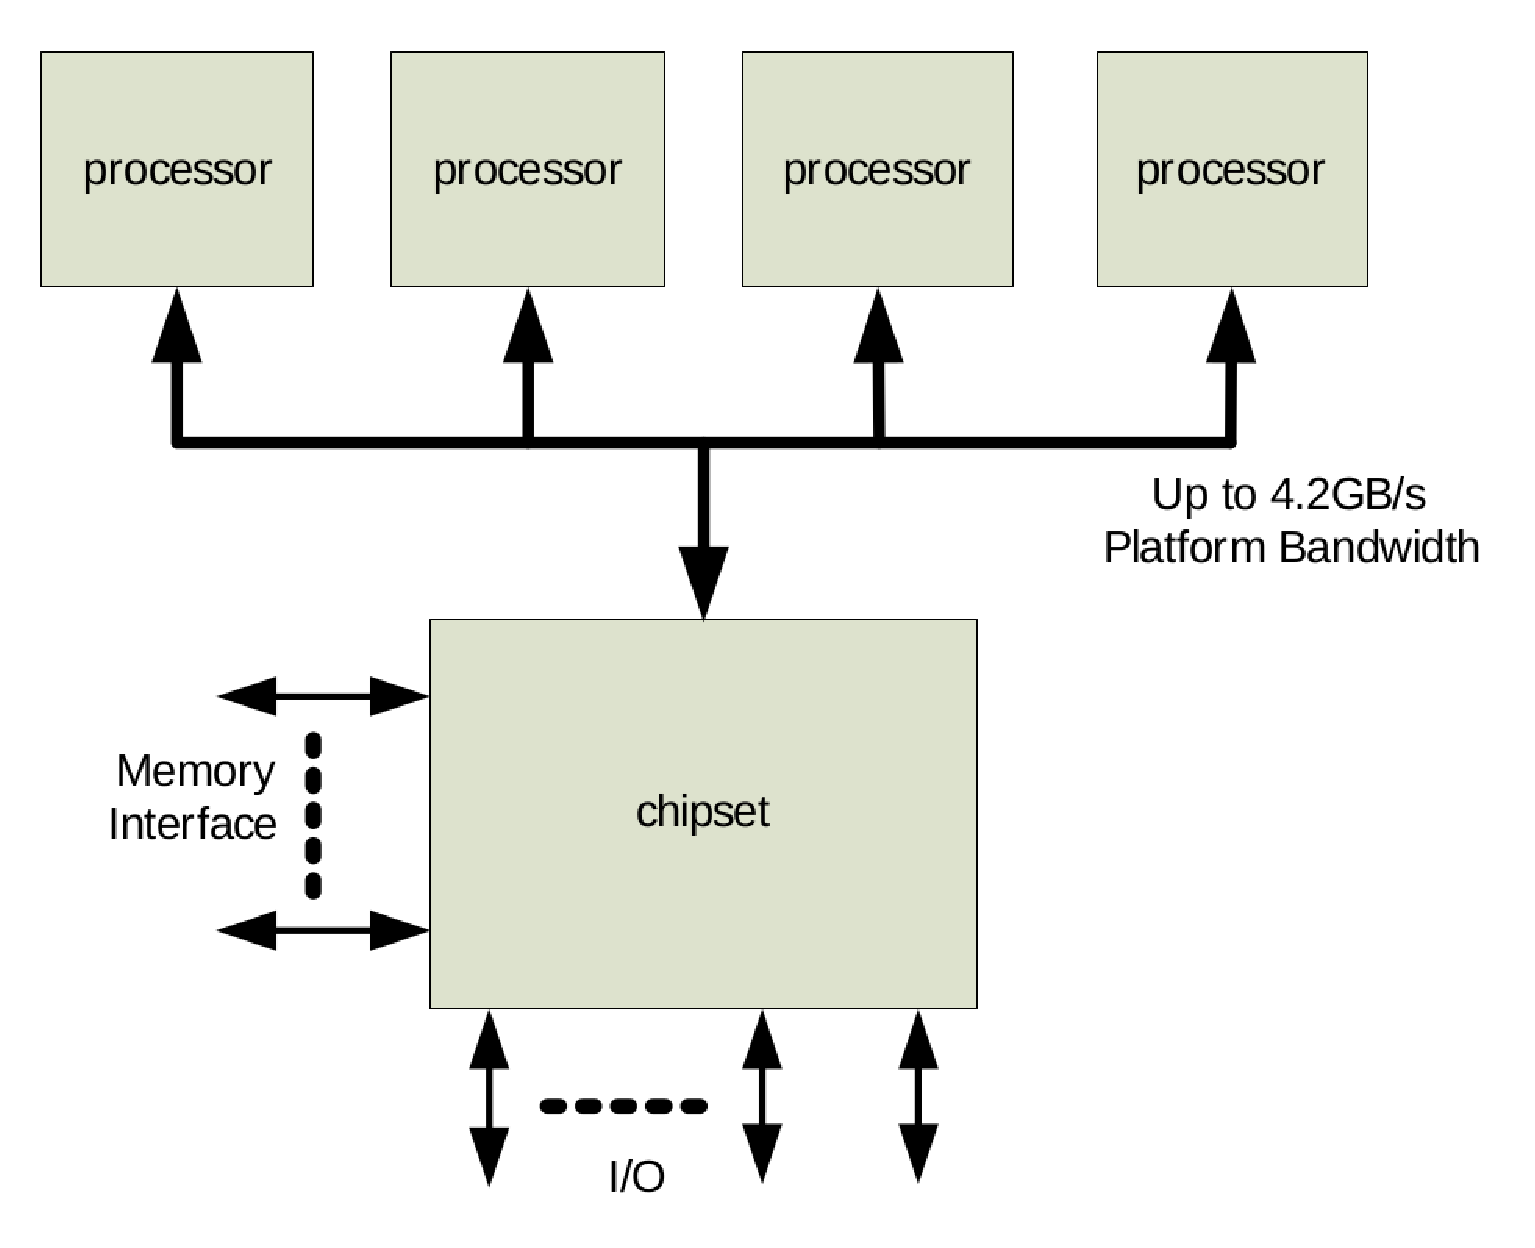
\includegraphics[width=.6\textwidth]{figures/uma1.eps}
		\caption[basic-uma]{Basic UMA System with the Frontside Bus as an unifying element. Image Intel Corporation \cite{qpi-intel}. }
		\label{fig:uma1}
\end{figure}

In situations where the power of a single processor computer is not enough -even if this processor is a multicore- it might be possible to incorporate in a computer system multiple processor chips. Usually in such multichip systems all the memory can be accessed by any of the participating processors. As the cores see a global memory space, it is possible that two processes access the same memory location at the same time. In this simultaneous access case it is advisable that when one processor writes over a memory location the other processors -even the ones located in other chip- see this change as well. This concept of keeping a synchronized version of a shared memory location is known as \textit{cache coherency}. 

In earlier multiprocessor systems the sharing of data between processors was done through a connection to the Front Side Bus, where memory can be accessed through the chipset (Northbridge) as shown in the Figure \ref{fig:uma1}. This shared bus topology meant that all memory accesses are treated equally no matter which processor accesses it, thus guaranteeing properties such as the latency of an access. This equality of accesses leads that this type of interconnection is known as an \textbf{Uniform Memory Access}. Later some enhancements were made to this architecture such as the segmentation of the shared buses and joining of these separate buses through cache coherency enforcement hardware \cite{qpi-intel}.

\subsection{Numa systems}\label{subsection:numa}

\begin{figure}
	\centering
		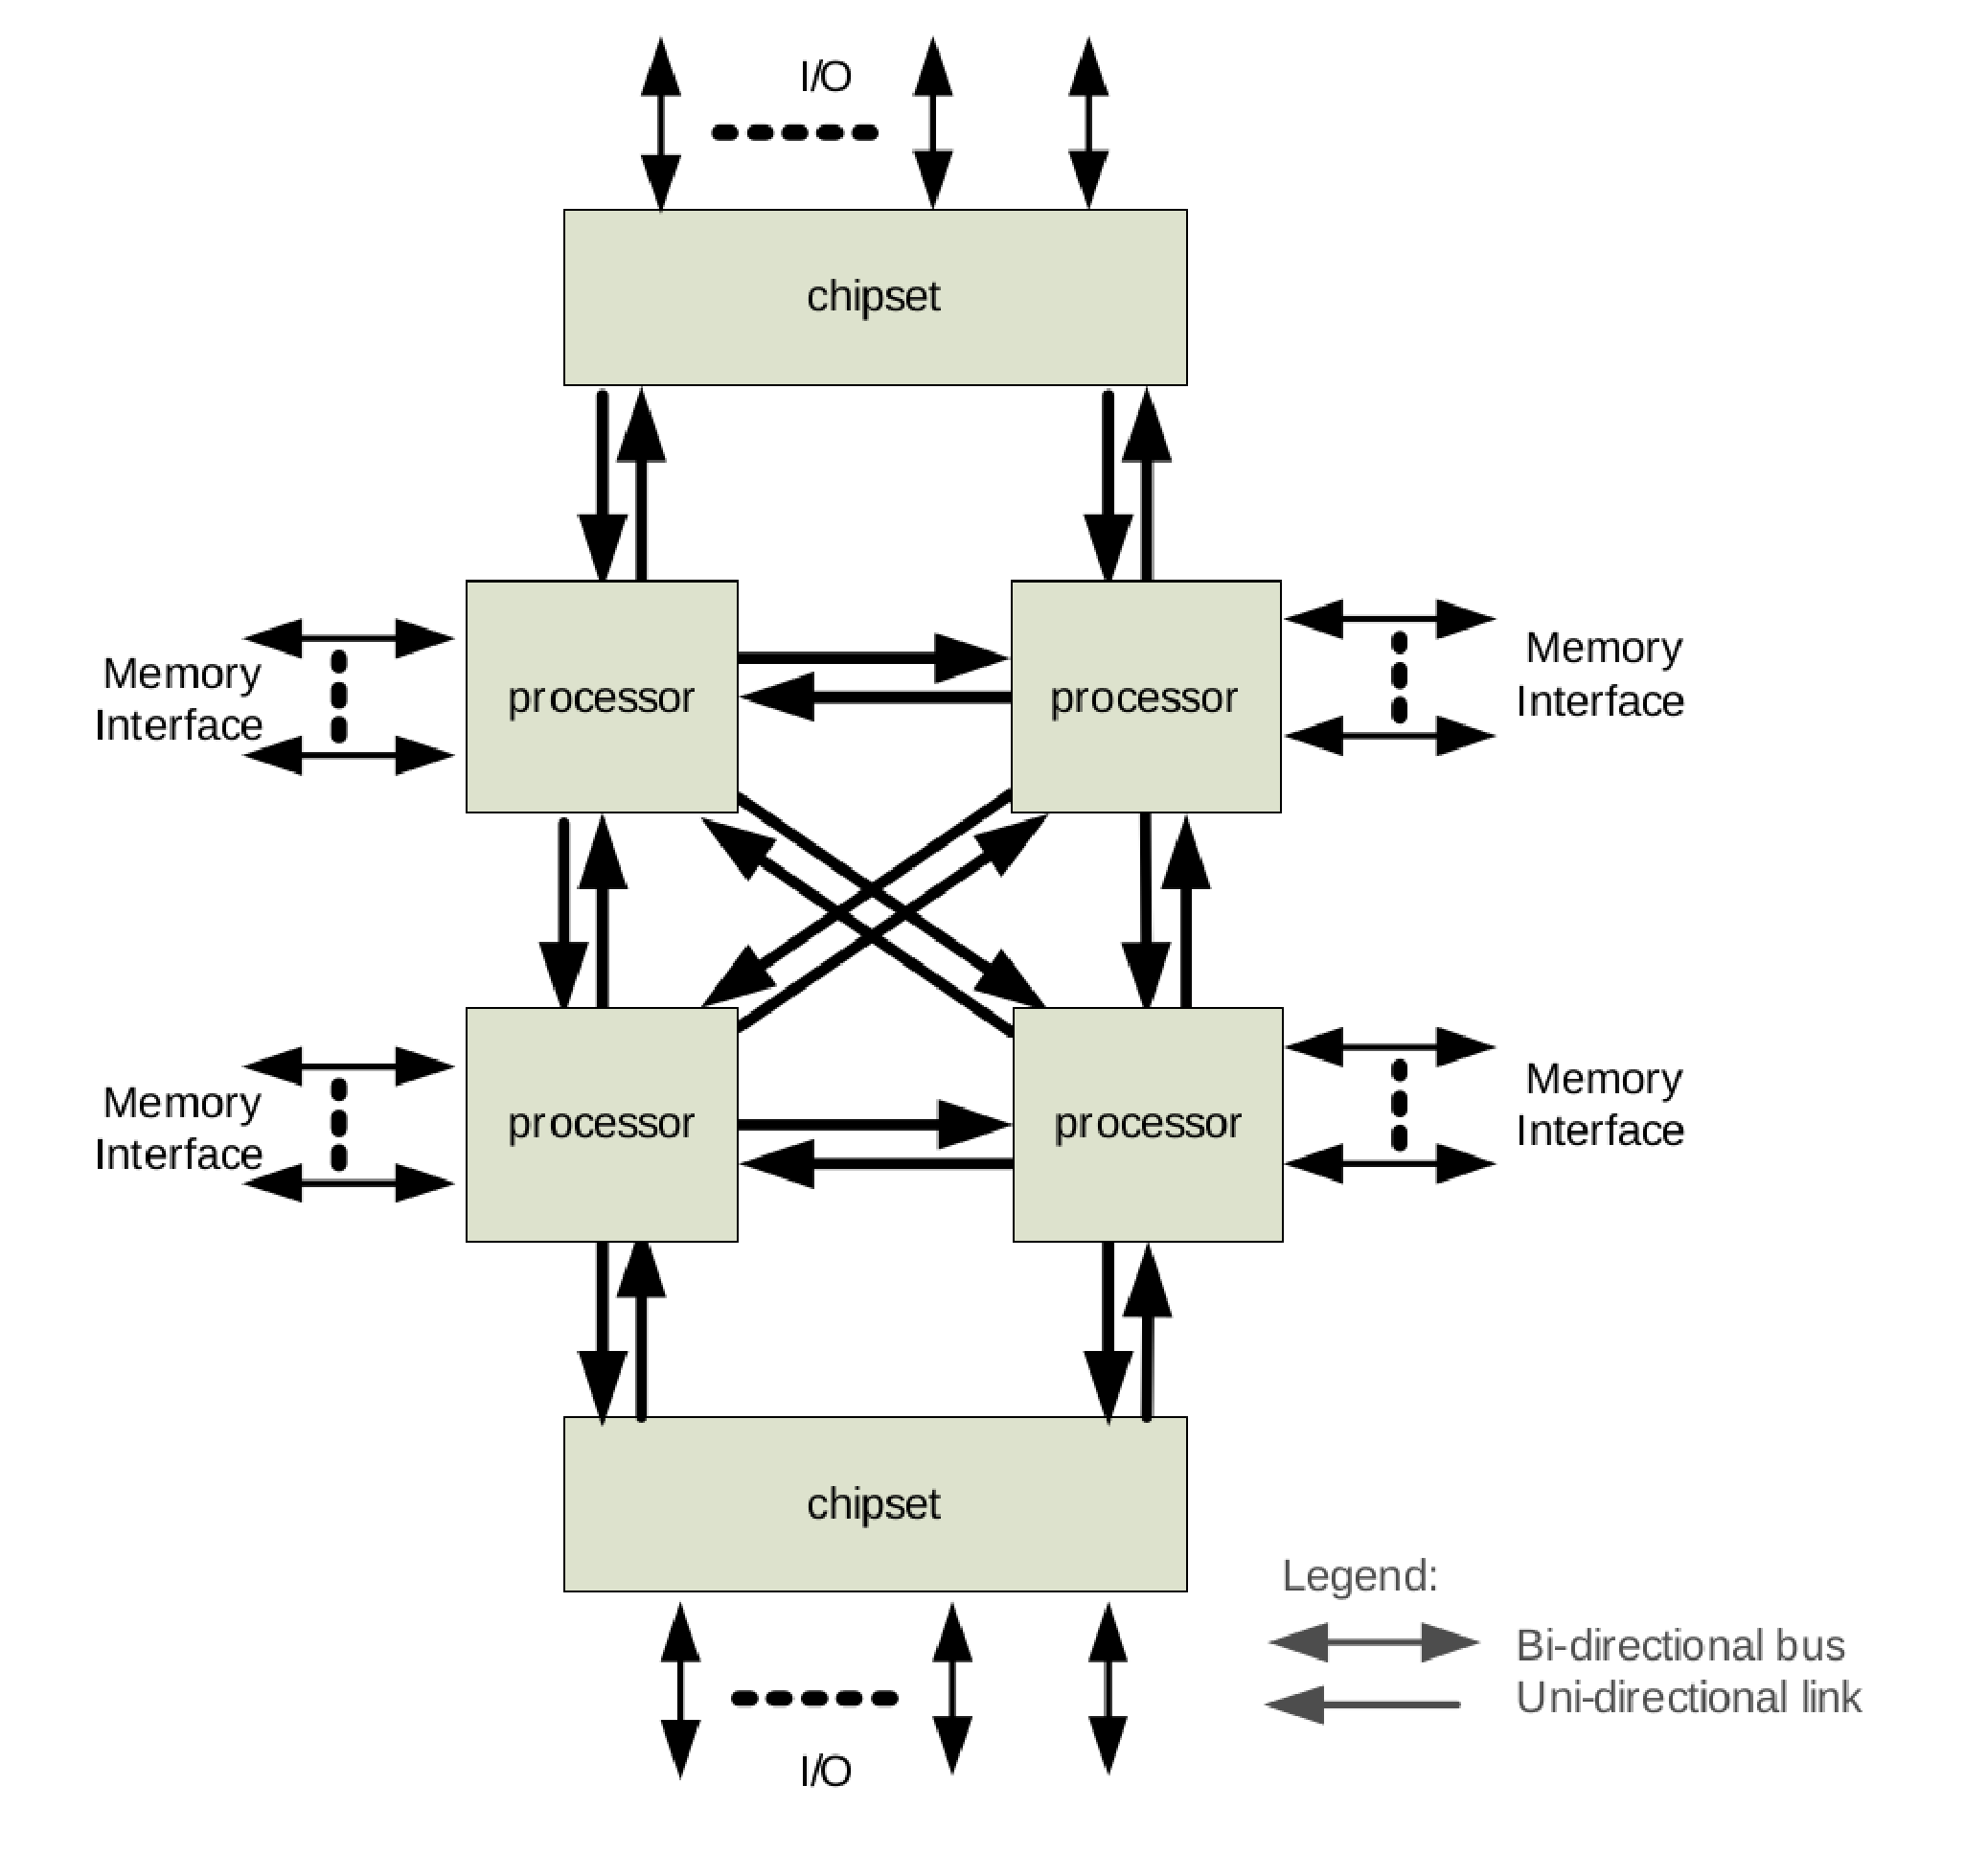
\includegraphics[width=.6\textwidth]{figures/numa-qpi.eps}
		\caption[basic-uma]{Numa system with four nodes with a QPI interconnection. Image Intel Corporation \cite{qpi-intel}. }
		\label{fig:numa1}
\end{figure}

Although the interconnection through the Front Side Bus provides very firm guarantees about the access time it has a very obvious downside, which is the bottleneck that could be produced when all the memory accesses are conducted through a single path. This bottleneck, together with the need to give the processor more memory access bandwidth with less latency has led to the development of point to point connection between processors. Instead of being just a bus protocol, these processor-memory links have taken the form of a layered protocol with packetized units of communication specific to every manufacturer. The most common forms of this new interface are Intel's Quick Path Interconnect and AMD's HyperTransport technologies. Figure \ref{fig:numa1} shows the representation of an Intel NUMA system interconected using QPI.

With the introduction of the point to point interconnects a processor faces two options when given the task of making a memory access: either the desired location resides in its attached memory or it must fetch the location from a remote processor. A remote memory access has more latency than a local one due to the interprocessor transport involved in the transaction, which leads to remove the guaranteed access latency given in the UMA system. This latency guarantee cannot be held anymore because of the placement of the threads and memory pages in a multiprocessor system can be easily changed thus introducing the NUMA architecture, which stands for: \textbf{Non uniform memory access}. 

\section{Computer performance measurement}\label{section:perfmeas}

Modern computers are complex systems and there are multiple factors that might contribute to a degradation in system performance. The addition of performance counters, as they are usually called, allows to help track occurrences that happen inside a processor and reading them facilitates the analysis of where a bottleneck could be taking place. These occurrences can be for example cache or TLB misses, memory loads or instructions retired from the pipeline, among others. The performance tracking facilities are also referred to as the \textit{Performance Management Unit (PMU)}.

In modern CPUs the number of available counters is fixed and every counter is programed by assigning it an event such as the ones mentioned above. The set of available events for every processor varies depending on the microarchitecture. 

\subsection{Instruction sampling}\label{subsection:sampling}
In the performance analysis of an algorithm sometimes it is desirable to associate the occurrence of an event with the instruction that caused it. Due to the great number of instructions executed by a processor it is not possible to keep track of every one of them. The strategy to apply here is to register information every certain number of instructions and extrapolate the results to the execution of the whole program. This follows the principle of \textit{Statistical Sampling} and thus it is called the \textbf{instruction sampling}.

The first sampling versions of instruction sampling that appeared in Intel and AMD processors sometimes had trouble with associating the exact event measured with the instruction in a precise manner, which caused a deviation in the association between the instruction and the event. Later, a revised version of the technology eliminated this shortcoming and it is present in current AMD and Intel processors with the proprietary names of \textit{Instruction Based Sampling} \cite{amd-ibs} and \textit{Precise Execution Based Sampling}  respectively. 

\subsection{Accessing the performance counters from code}\label{subsection:accessing-code}

There is no direct API provided to access the information contained in the access counters and due to the information that some counters expose in many cases, this access can only be performed just by code that executes in system mode.

In Linux, which is the operating system chosen for the implementation of the solution, the access can be done through the perf facilities implemented in the kernel. There is a system call that allows to configure the counters to be used and the resulting readings can be retrieved by reading to a memory location. For a more detailed description of the access to the counters through perf, refer to the section \ref{section:ovv-perfks}. 

\subsection{Documentation of the performance measurement facilities: The Intel case }\label{subsection:performance-documentation}

Every processor equipped with performance counters has the description of these facilities in the operation manuals. In the case of Intel, the relevant information can be found in the chapters 18 and 19 of the System Programming Guide \cite{intel-devguide}, although there are separate documents which extend this information, such as the uncore performance monitoring guides. The availability and layout of performance information is not architecturally uniform, this means that every microarchitecture, even from the same architecture family, has very specific performance measurement features that might differ from other microarchitectures.

One of the examples of these difference between microarchitectures is the case of the registers, those who are present in all the architectures such as the EAX registers are named Architectural registers and those that change through the changes in architectures are called \textbf{Model Specific Registers}, or MSRs. Chapter 18 gives an account of the performance measurement features present in every processor family and chapter 19 gives the concrete event information for all the events available.

Following this separation of architectures, these chapters present an overview of the performance measurement in Intel processors and then all the specific information for every microarchitecture family is presented separately. Usually, in order to make use of a counter we need to program it with the identifier of the event we are interested on, together with some additional information, if necessary.

All the information about bit fields in this project is ignored, because such low level is not needed and the low level access to the registers will be performed by the kernel side of perf. For us it will be necessary only to fill a struct with some fields that specify the events we want to read.
\begin{table}
	\centering
		\begin{tabularx}{\textwidth}{|l|X|}
		\hline
			Event Num & CDH\\
			\hline
			Umask Value & 01H\\
			\hline
			Event Name & MEM\_TRANS\_RETIRED.LOAD \_LATENCY\\
			\hline
			Definition & Randomly sampled loads whose latency is above a user defined threshold. A small fraction of the overall loads are sampled due to randomization. PMC3 only\\
			Description and comment\\
			\hline
		\end{tabularx}
		\caption{Description of the load latency record event as it appears on the Intel manual}
		\label{table:lldescr}
\end{table}
For example, in the case of the Sandy Bridge microarchitecture, we will be using an event called the \textbf{load latency record}, which is defined in table 19.9 of such guide. Table \ref{table:lldescr} gives an example of the information contained in the event reference. The identifier of the event to be measured is given by the event number together with the umask value, the definition provides a definition of what the event measures and the description and comment field indicates that for this case additional information can be specified, such as the minimum weight that a sample must have in order to be passed to the software .

\section{Related software}\label{section:relatedsw}

\subsection{Libnuma}\label{subsection:libnuma}

Libnuma \cite{libnuma} is one of the most important libraries for the control of NUMA systems. Among its most important features it incorporates the ability to control the processor and memory mappings of a process within a NUMA context.

Of particular importance to this project is the \texttt{move\_pages} call, which allows to determine in which node a given memory page is and commands the move of the desired memory pages from one node to another. Many of the functionalities offered by libnuma are available as console invocable commands by using the \textit{numactl} application. Numactl also provides a quick way to discover the NUMA layout of a processor by using the \texttt{--hardware} argument.

%--NICE2HAVE= Ex of numactl --hw using bulldozer 
\subsection{Autopin and Autopin+}\label{subsection:autopin2}
Autopin is a tool developed by the chair of computer technology and organization of the Technical University of Munich \cite{autopin}. As explained in the introductory section the pinning or mapping of the running threads to the available cores can be crucial to obtaining good algorithm runtime performance. When the optimal pinning of an application for a given system is not known, a good approach is testing many alternative pinnings to find out which one helps the application perform better, which is precisely the way Autopin works.
For Autopin to work, the process to run and the alternative pinnings to be tested are given as an input. On execution Autopin will run the requested process or attach to an existing one, try the different pinnings for a certain amount of time and when all the pinnings are tried stick to the best alternative in terms of performance. For performance measurement Autopin will calculate the performance rate as a ratio between the difference of two PMU readings and the time the program was allowed to run under a certain pinning. The PMU readings are related to the number of instructions executed and are taken at the beginning and end of the measurement period. Before the measurement of the performance rate and the set up of an specific pinning there is a period of time that the program will be allowed to run without making any measurement, this interval will be referred to as the warm-up period.

\subsection{Software for performance measurement }\label{subsection:software-pm}

Currently there are many alternatives for accessing the performance information and even for analyzing it in order to formulate diagnostics about the performance of the program. This section aims to briefly indicate some ready to use alternatives present in the market:

\begin{itemize}
	\item Intel VTune: Closed source licensed tool which features a rich graphical interface and advanced diagnostics capabilities. Only available for Intel processors.
\item Perf: Performance measurement implementation for the Linux kernel. It features the ability to access performance information for multiple processor architectures. Provides an interface to create user space programs that process the measurement information.
\item Intel Performance Counter Monitor: Open source tool which provides facilities to access the CPU performance counters facilities as a C++ API. Only available for Intel processors and for many features requires root access.
\item Intel NumaTop: Open source tool that follows the principle of the Linux Top Tool. Instead of providing information of the CPU utilization provides information of how much remote and local bandwidth each process is making use of, together with other information such as information of the allocation of memory and measurement of the average memory latency. Only available for Intel processors. 
\end{itemize}

\subsection{An introduction to perf }\label{subsection:intro-perf}

Perf has become one of the most important tools for accessing the CPU performance information, its code has been incorporated into the Linux source three. Unfortunately the code is scarcely documented and the best way to learn its workings is through the analysis of the implementation and the reading of the repository commits. Although perf belongs to the kernel source tree it is not necessary to compile a kernel to generate a working version of the user side of perf because it contains its own Makefile.

Perf is divided in two parts, the Kernel side and the user tools: The kernel side takes care of the direct communication with the Performance monitoring unit and providing a representation of the performance data independent of the underlying architecture and even different microarchitectures of the same processor family. The user side contains a set of tools which allow to gather the performance information and perform different analyses. There is also the opportunity to create a custom user side that relies on the kernel side, which is the approach that will be taken during the development of this project. The specific aspects of invoking the kernel side will be discussed in section \ref{section:ovv-perfks}.

Perf not only allows to access the performance information given by the CPU, but also allows to access performance information that is stored in the kernel, for more information type \texttt{perf list}. The system administrator must tune the \texttt{perf\_event\_paranoid} setting depending on how much access he wants the regular user to give. 